\documentclass[11pt, english]{article}
        \usepackage{geometry}
                \geometry{
                        a4paper,total={210mm,297mm},
                        tmargin=32mm,
                        bmargin=32mm,
                        lmargin=24mm,
                        rmargin=24mm,
                }

	\usepackage{titlesec}
                \titleformat{\section}
                        {\normalfont\fontsize{18}{16}\bfseries}{\thesection}{0.5em}{}
                \titleformat{\subsection}
                        {\normalfont\fontsize{14}{16}\bfseries}{\thesubsection}{1em}{}
                \titleformat{\subsubsection}
                        {\normalfont\fontsize{11}{16}\bfseries}{\thesubsubsection}{1em}{}

	\usepackage{float}

	\usepackage{longtable}
        \usepackage{multirow}

	\usepackage{caption}
                \captionsetup[table]{labelfont=bf,textfont=bf,font=small,skip=8pt}
                \captionsetup[figure]{labelfont=bf,textfont=bf,font=small,skip=8pt}
        \usepackage{subcaption}
                \captionsetup[subtable]{labelfont=rm,textfont=rm,font=small,skip=8pt,labelformat=parens,labelsep=space}
                \captionsetup[subfigure]{labelfont=rm,textfont=rm,font=small,skip=8pt,labelformat=parens,labelsep=space}

	\renewcommand{\thetable}
                {\thesection.\arabic{table}}                                                         
	\renewcommand{\thesubtable}
                {\roman{subtable}}

	\renewcommand{\thefigure}
                {\thesection.\arabic{figure}}
        \renewcommand{\thesubfigure}
                {\roman{subfigure}}

        \usepackage{hyperref}
                \hypersetup{
                        colorlinks=true,
                        linkcolor=black,
                        filecolor=magenta,
                        urlcolor=cyan,
                        }

        \setlength{\parindent}{0pt}
        \renewcommand{\baselinestretch}{1.25}
        \usepackage{setspace}

        \usepackage{amsmath}
        \usepackage{amssymb}

	\usepackage{graphicx}

	\usepackage{tikz}
                \usetikzlibrary{trees,arrows,topaths}

	\usepackage[utf8]{inputenc}
	\usepackage[T1]{fontenc}

\begin{document}

\pagenumbering{gobble}

	\title{\textsc{CS993 Software Engineering\\ Coursework Assignment}}
	\author{\textsc{Group 2}}
	\date{\textsc{Academic Year 2021/2022}}
        \maketitle

\newpage

\pagenumbering{roman}

	\renewcommand{\contentsname}{Table of Contents}

	\tableofcontents

\newpage

\pagenumbering{arabic}

\section{Introduction \& Background}

	The system featured in this project is a cinema booking system which allows interaction of three tiers of users: administrators, cinema staff, and cinema-goers. In-line with the brief of this project, administrators take on the outlined \textit{administrator} role, where they are able to create \textit{projects} and \textit{tasks} and assign other users to these. However, both cinema staff and cinema-goers are considered `bookers'. Cinema staff hold the most relevant role (to the brief) in this case, where they are able to be assigned to \textit{projects} and \textit{tasks}, book time periods, and add notes, etc., relevant to the cinema context. The cinema-goers are able to book film showings in theatres, which have been generated using the former user types. This is more of a formality.\\

	This project contains various layers including GUI aspects and rear-end data management which, although applied in a simple context, can become confusing if not correctly and efficiently projected. Thus, appropriate project planning and management elements and principals have been utilized throughout the development process and will be portrayed in this report.

	\subsection{Client \& Users}

	Our client throughout this project is Eclipse Cinemas, a local cinema operator. They tasked us with creating a system that could be deployed across their cinemas. From the offset, they had two primary requirements for the system: to provide an online system for their customers to view and book films; and to provide a system to help cinema staff manage their daily tasks.

	There are two implied targets for this piece of software: cinema management teams and cinema-goers. Of course in the real world, these systems tend to be kept apart with the staff management system relating to and only being available for corporate use; and, the separate booking system being managed by a relevant development team and information being relayed to the cinema staff. However, in the case of this basic system and the associated brief, keeping corporate-use and commercial-use abilities within one program creates harmony between the elements.

	\subsection{Development Process}

	Generally, the development process of the system featured in this project follows the chain of: requirement analysis $\rightarrow$ structural design $\rightarrow$ graphical user interface functionality $\rightarrow$ rear-end data management system functionality and connectivity $\rightarrow$ graphical user interface graphic design $\rightarrow$ testing. As this system involves features such as log-in and booking capabilities and distinctions as well as a neat but slightly Soy user interface, various languages are utilized, including: HTML, CSS, SQL, and JavaScript. A large portion of this development took place using Bram Moolenaar's Vim.

\newpage

\section{Requirements}

	Clear and comprehensive requirements form the foundation and act as a guide in the completion of every software project. They define the features that the software is expected to include and produce, and usually evolve as the project evolves. In the case of this project, a list of requirements were initially identified by the client which detailed an application which facilitated various users of a cinema system accessing features that enable user-specific functionality. The requirements were documented and incrementally delivered to the client for validation and verification with regular communication facilitated by online meetings using Zoom.\\

	Our team adopted an Agile style of working with numerous methods of communication, including a virtual Zoom meeting room which are further discussed in the Project Management section of this report. As always, additional requirements emerged and were added to the application accordingly throughout subsequent iterations.

	\subsection{MoSCoW Methodology}

	Upon initiation, requirements were divided into \textit{functional} (what features the software is expected to have) and \textit{non-functional} (the behaviour of the software, including restraints). Accurate analysis and documentation of these requirements were performed using the MoSCoW methodology. This offered an effective prioritization technique which, with input from stakeholders, classified the client's requirements into the following features and functionality:

	\begin{itemize}
	\setlength\itemsep{0cm}
		\item \textbf{Must-have} features which detail the absolutely necessary and basic functionality for the software to become a viable product.
		\item \textbf{Should-have} features which should be considered once the must-have features are satisfied. They offer additional functionality and should be included immediately in the following iteration.
		\item \textbf{Could-have} features which follow-on from the should-have features and offer optimization of the product functionality.
		\item \textbf{Won't-have} features which focus on requirements that won't be included in time for the completion of the project for reasons which may extend to: time constraints, technical skill limitations, financial constraints, etc.
	\end{itemize}

	\subsection{Functional Requirements Documentation}

	The client provided an initial set of requirements that were further developed, verified and incrementally delivered back to the client for validation throughout the life-cycle of the project during a series of virtual meetings. Our team, of course, were tasked with creating a cinema management and booking system which was prioritized as outlined below.

		\subsubsection{Validation and Verification: Initial Must-Haves}

	All users must have the ability and scope to observe:

	\begin{itemize}
        \setlength\itemsep{0cm}
		\item Distinguish visually between cinema staff and customer interface
		\item Ensure color scheme is accessible
		\item Visuals should be consistent across multiple devices
		\item Usability and accessibility features included
		\item The system must allow all user types to create an account
		\item Users (administrators, staff and customers) are assigned specific access rights and features accordingly
		\item Users are able to use the system to create, be assigned to, interact with and books projects / tasks
	\end{itemize}

	and specifically, administrators must be able to:

	\begin{itemize}
        \setlength\itemsep{0cm}
		\item Create and update films and their attributes
		\item Delete films
		\item Assign showing times to films
		\item Assign theatre screens to films
		\item Update account details
		\item Create a \textit{Staff} user account for staff
		\item Assign shifts to staff users
	\end{itemize}

	and, staff must be able to:

	\begin{itemize}
        \setlength\itemsep{0cm}
		\item View assigned tasks
		\item View shifts
		\item Mark tasks as complete
	\end{itemize}

	and, customers must be able to:

	\begin{itemize}
        \setlength\itemsep{0cm}
		\item View available films
		\item Book ticket(s)
		\item Be notified of a booking confirmation (with unique identifier) on-screen
	\end{itemize}

		\subsubsection{Validation and Verification: First Iteration - Should Haves}

	The requirements were verified and validated by the client during a routine scheduled meeting and further requirements were raised. These formed the focus of features for the next iteration.\\

	Administrators should have the ability to:

	\begin{itemize}
        \setlength\itemsep{0cm}
		\item Manually block and reserve theatre seats
		\item Update current film listings and their attributes
		\item Assign projects/tasks to \textit{Staff} users
		\item Simulate a \textit{Staff} user overview of all tasks assigned
	\end{itemize}

	and, staff should be able to:

	\begin{itemize}
        \setlength\itemsep{0cm}
		\item Add comments to tasks to which they have been assigned
		\item Create new tasks at request
	\end{itemize}

	and, customers should have the ability to:

	\begin{itemize}
        \setlength\itemsep{0cm}
		\item Select seats for themselves
		\item Not have the ability to reserve seats being viewed by other customers, at their time of viewing
	\end{itemize}

		\subsubsection{Validation and Verification: Second Iteration - Could Haves}

	Upon completion of the second iteration, another meeting with the client verified the features raised in the first validation meeting and offered the team further insights into additional requirements which were not clearly defined in the initial subsequent requirements request. Maintaining close communication with the client enabled the team to identify further features and the requirements which must be aligned in the final iteration for the optimization of the application. These formed the focus on the could-have requirements.\\

	Customers could have the ability to:

	\begin{itemize}
        \setlength\itemsep{0cm}
		\item Receive an e-mail confirmation of booking
		\item Search for films and their attributes using a search function
		\item Rate a film feature
	\end{itemize}

		\subsubsection{Validation and Verification: Third Iteration - Won't Haves}

	Upon our team's final meeting with the client for validation and verification, various features were highlighted which were not included in the final system prototype to-date as they were outwith the scope of the project given the discussed constraints. The features which won't be included in the system would have focused on optimization of the \textit{Staff} and \textit{Customer} users. It was crucial that the prioritization of the requirements was correct and coherent to ensure an efficient, high-quality and viable product. Non-functional requirements were also apparent from the user requirements and are explored subsequently.\\

	Hence, customers won't have the ability to:

	\begin{itemize}
        \setlength\itemsep{0cm}
                \item Watch a film trailer
        \end{itemize}

	and, staff won't have the ability to:

	\begin{itemize}
        \setlength\itemsep{0cm}
		\item Request specific shifts out of all of the available time slots (only request low-scope amendments)
		\item Request annual leave (or any other form of geographical norm)
        \end{itemize}
	
	\subsection{Non-Functional Requirements Documentation}

	The non-functional requirements of this system were discussed with the client and centered around security, time constraints and access rights. These were all prioritized using the MoSCoW method and it was decided that all non-functional requirements were to be included and implemented in time for the second iteration. So forth:

	\begin{itemize}
        \setlength\itemsep{0cm}
		\item Users have access rights and features which are restricted to their specific user type (must-have)
		\item An appropriate and secure database management system to store and authenticate user log-in and personal details is included (must-have)
                \item Time constraints on loading between pages are included to ensure development methods adhere to efficient formatting
        \end{itemize}

	\subsection{Usability and Accessibility Requirements}

	The team focused on creating a user-centered application which included usability and accessibility features as part of the core design. This resulted in a user-friendly GUI which users found easy to navigate. This application uses a suitable font size with clear and concise language and linguistics leading to eased comprehension, and industry standard icons for easy recognition leading to faster navigation. Suitable but relevant and appealing color combinations with appropriate contrast levels were also implemented. Involving users and conducting multiple tests during the development process (UAT and focus groups), enhanced the optimization and success of the application and limited user dissatisfaction.

	\subsection{User Stories}

	Our team used user stories as part of our refinement of requirements protocol. These stories guided the prioritization of functional requirements giving a description of the actions needed to perform a task from the user's perspective. The following show a sample of the user stories identified by the team:

	\begin{enumerate}
        \setlength\itemsep{0cm}
		\item As user: `I want to create an account' (must-have)
		\item As user: `I want to be able to update details on my account' (must-have)
		\item As customer: `I want to book (a) ticket(s)' (must-have)
		\item As customer: `I want to receive confirmation of my booking via e-mail' (must-have)
		\item As administrator: `I want to create and update films and their attributes' (must-have)
		\item As administrator: `I want to create staff users and assign them shifts' (must-have)
		\item As staff: `I want to view my shifts' (must-have)
		\item As staff: `I want to view my current tasks' (must-have)
        \end{enumerate}

	\subsection{Backlog Refinement}

	Implementing backlog refinement throughout the project provided a useful way in which the team could maintain focus on the most important user stories which aligned with each iteration of the system development. In performing regular backlog sessions, the team were able to maintain an open line of communication between stakeholders, reduce the risk of unexpected outcomes and provide feedback to each other and the client to ensure the development of optimized and viable software.

\newpage

\section{Project Management}

	The end goal for this project was to successfully deliver an operational system to the client by the 18th of March. Therefore, we developed a string project management plan to ensure this goal was fulfilled.

	\subsection{Visual Planning}

	The first step in our project planning was to identify the key milestones which must be reached on the path to achieving our final goal. Working backwards from the delivery date, we assigned realistic deadlines for each milestone; allowing sufficient tolerance allocated to events such as unforeseen delays and avoidance of overwhelming pressure on the team. We represented the full project plan using a Gantt chart. This served as a strong visual representation which could be referenced consistently throughout the development process, and allowed the team to easily track the deadlines and responsibilities of each project segment. The chart was not a fixed piece as it was altered throughout the process when particular tasks required duration amendment, for example, to achieve our desired results. This is outlined in the figure below.

	\begin{figure}[H]
	\begin{center}
		\includegraphics[width=16cm,height=5.5cm]{CS993_IMG/GANT_Section.pdf}
		\caption{Gantt Chart}
	\end{center}
	\end{figure}

	To aid our planning, we visually represented the development of our system's key components on a PERT chart. This served as a reference in each sprint to help refine the workflow and maintain focus on the project's primary path. While all elements of the chart were not relevant to every sprint, the overarching journey remained the same through each iteration. This is outlined in the figure below.

	\begin{figure}[H]
	\begin{center}
		\includegraphics[width=16cm,height=5.5cm]{CS993_IMG/PERT_Section.pdf}
		\caption{PERT Chart}
	\end{center}
	\end{figure}

	\subsection{Collaboration}

	To `kick-start' the project, we held an initial meeting to develop the overarching concept for our system. This also marked the beginning of the requirements gathering process which is documented elsewhere. From the outset, roles were assigned to each member of the team which utilized each person's unique strengths and skill-set.\\

	So forth, David and Lewis were respectively assigned responsibility for back-end and front-end development, and testing. Camille and Declan took charge of project management, and requirements gathering and maintenance/documentation, respectively.\\

	Following the initial briefing session, weekly progress meeting were conducted throughout the development process. We used this time to update all team members on each individual's progress, and to highlight any issues encountered to be reviewed. These meetings were also used to tackle group-wide tasks such as requirements brainstorming, refinement and prioritization.

	\subsection{Tools}

	To support our project management goals, the team utilized several tools and technologies. The discussed weekly progress meeting were held on Zoom, which was also used for more irregular or impromptu catch-ups and collaboration between particular team members. We created a Facebook Messenger group which was used for regular text-based communication throughout the project.\\

	We utilized the project management software Asana to structure and manage our defined tasks in a central space. We created a `project board' which acted as a visual aid in tracking tasks and their assignment to team members. This provided an easy reference for planning and delegating which allowed all team members to be fully aware of the progress within the system development and reporting.\\

	For documentation, the team used Microsoft's SharePoint to provide a shared space which allowed all team members to access the full workflow at all times. And, to allow spontaneous amendments and collaboration. The final report however, is of course typeset using Donald E. Knuth's \LaTeX\ in Bram Moolenaar's Neo Vi Improved.\\

	On the development side, the team used GitLab to store and share code for the user interface (front-end) and data management system (back-end). This of course, like documentation, also meant collaboration was easily possible. Using a version management system such as this provided an extra layer of security in monitoring the system's progress, enhancements and errors.

	\subsection{Software Life-cycle}

	We used Agile methodology in the process of the software development. We considered the Waterfall method but felt this was too constricting for our purposes. The flexibility and room for rapid alterations and improvements provided by Agile promised a better fit for the team's goals.\\

	We cycled the project in three `sprints', each with a two-to-three-week duration. Within each sprint, we adhered to the full range of the development life-cycle: requirements, design, development and testing. The primary advantage of this agile approach was highlighted by the fact that the team managed to produce a successful and viable product by the end of each sprint.\\

	Our first sprint focused on implementing all of our `must-have' requirements. We began by adding any `should-have' and `could-have' requirements into succeeding sprints alongside the `must-have' requirements which emerged throughout testing and analysis. These requirements are outlined in the previous section. A top-down summary of how they interact with the sprints is displayed in the following table.

	\begin{center}
		\scriptsize
	\begin{longtable}{p{14cm}}
		\hline
		\multicolumn{1}{c}{\textsc{First Iteration}}\\
		\hline
		All users can create accounts\\
		Accounts are authenticated and distinguished between different users (administrators, staff and customers), with different accessibility and functionality, accordingly\\
		Administrators can create, update and delete films\\
		Customers can view and book films, and receive onscreen confirmation of booking\\
		\hline
		\multicolumn{1}{c}{\textsc{Second Iteration}}\\
		\hline
		Administrators can update the current movie list and block/reserve specific seats\\
		Administrators can see an overview of all tasks from the perspective of themselves and each member of staff\\
		Administrators can create staff user accounts and assign projects and tasks to them\\
		Customers can view and book specific seats of a film showing at a time in a theatre. They cannot book seats currently being viewed by other customers at their time of viewing\\
		Staff can request creation of new tasks and add comments to all of their assigned tasks\\
		Staff can view assigned projects, tasks and their duration, and mark these\\
		\hline
		\multicolumn{1}{c}{\textsc{Third Iteration}}\\
		\hline
		Customers can receive an email confirmation of a booking\\
		Customers can search for specific movies\\
		Customers can rate films they've attended a showing of\\
		\hline
		\caption{Software Development Iterations}
	\end{longtable}
	\end{center}

	Following testing the third iteration at the end of our third sprint, we executed one final round of revisions to repair any small but urgent issues which emerged in the testing process. Following that, the finished product was ready for presentation to the client.

\newpage

\section{Design}

	On a high level, this system is like many others; it allows user interaction (of various types) through an attractive interface on the front-end, it allows this interface to communicate with various non-complex computations and algorithms which translate to different manipulations of data on the rear-end, and it provides different user outputs and results based on the relevant data manipulation and requests. The design process of this project follows the standard `Agile' cycle, where client requirements are analysed, practiced and tested to explore feasibility. This concept is discussed in further detail in the project management portion of this report.\\

	After the identification of user requirements and consideration of their feasibility and relevance, it's important to gain an idea of how users will interact with the final product and what they will interact with. Therefore, there is little logic in immediately developing a rear-end data management system without an idea of data flow. The preliminary stages of the data flow are made clearer by prototyping and exploring opportunities relevant to the user interact. Not only is this an important process for gaining perspective of the scope of the proposed functions within the system, it also helps identify areas in which the program's scale can be moderated and adjusted relative to the project's time scale and developer capabilities etc.\\

	\begin{table}[h]
		\scriptsize
		\renewcommand{\arraystretch}{1.25}
	\begin{center}
	\begin{tabular}{lll}
		& \textsc{Language} & \textsc{Environment}\\
		\hline
		UI Functionality & HTML & CL/Vim\\
		& JavaScript & \\
		UI Graphic Design & CSS & CL/Vim\\
		Rear-End Functionality & SQL & CL/Vim\\
		& Python & \\
		\hline
	\end{tabular}
		\caption{Utilized Languages}
	\end{center}
	\end{table}

	As discussed previously, this is a multi-layer system which means it utilizes multiple layers of functionality, outlined in Table 3.1. This calls for skills in various areas of programming starting in the area of more `tangible' product-producing languages such as HTML in the UI functionality stage. Development in this areas arguably requires the greatest understanding of the target user and how they wish to functionally interact with the product; how they wish to navigate, what they actually want to gain from their specified requirements, etc. Furthermore, the UI graphic design stage requires a greater conceptual/artistic understanding of the target user, what's familiar, what's relevant to the industry, what just the right amount of a unique touch is to make the product stand out but not irrelevant, etc. Finally arguably the most important stage from the perspective of quality and longevity, the rear-end functionality. This requires the greatest understanding of how elements translate user interaction to the output delivered to the user.\\

	It's here where various aspects of the `Agile' process become relevant. The strengths of individual team members are tasks are identified and the three elements of this process are designated to the relevant members. This means that ideally each element is built to the team member's strengths and stages are completed efficiently. This therefore leaves plenty of time for the joining stage. Due to the ongoing use of a version control system, all team members stay well informed so collaboration is not a hassle.

	The decision is already made in the context of this project; the user must interact with this application through a web browser or mobile application etc. In other cases, decisions must be made regarding the location of the input/output. For example, will the program be terminal-based? Or will it have a graphical user interface? On what and which type of platform will it be available?\\

	In the case of this project, this step involves segmenting the system into portions relevant to each type of user, as outlined in Table 3.2. Thus, creating a system (in this case, log-in) which directs users to their intended target. Of course the process of executing this is more relevant when user data is analysed on the rear-end. Once users arrive at their correct destination, each group must have a unique set of abilities (pages) and options (functions). For example, allowing administrators to create and manage events (staff \textit{projects} and movies etc.) around the cinema; allowing staff to be assigned to \textit{projects} and nominate themselves for \textit{tasks} managed by administrators; and, allowing bookers to view and book movie viewings created by administrators. HTML, JavaScript and Python make these interactions tangible however, they are only functional when combined with the rear-end data management.

	\subsection{User Interface Graphic Design}

	The graphic design of a system's interface is often an overlooked aspect, especially in smaller development teams where specialization or skill in the graphic communication and publication design field may be limited. Thus, this aspect is often outsourced in larger commercial environments. However, the product must look good if users are expected to voluntarily communicate with it time after time. The brand and product must be displayed effectively through the elements and principals of graphic design, in order to fully engage the consumers.\\

	In this context of cinema, there must be relevance to not only the existing content on the market, but also to content which correctly portrays the scale and scope of the film industry. More specifically, the interface must also be relevant enough in particular areas in order to differentiate between the corporate side of the system (admin and staff) and the commercial side (public booking). 

	\subsection{User Interface Functionality}

	To fulfil the functional and non-functional requirements discussed, the program approximately takes on the structure as follows (and is further discussed in the chapter succeeding this one):

	\begin{center}

	\tikzstyle{level 1}=[level distance=1cm, sibling distance=4.5cm]
        \tikzstyle{level 2}=[level distance=1cm, sibling distance=2cm]
        \tikzstyle{level 3}=[level distance=1cm, sibling distance=1.5cm]
        \tikzstyle{level 3}=[level distance=1.5cm, sibling distance=1.25cm]

        \tikzstyle{bag} = [text width=5em, text centered]
        \tikzstyle{end} = [text width=7em, text centered]

        {\scriptsize\begin{tikzpicture}
                \node[bag] {Log-In}
                        child {
                                node[bag] {Administrator}
                                        child {
                                                node[end] {Add\\Film}
                                                        child {
                                                                node[end] {Details,\\Theatre,\\Remove Film}
                                                        }
                                                }
                                        child {
                                                node[end] {Manage\\Project}
                                                        child {
                                                                node[end] {Staff Shift,\\Element / Time}
                                                        }
                                                }
                                        child {
                                                node[end] {Add\\Staff}
                                                        child {
                                                                node[end] {Details,\\Role}
                                                        }
                                                }
                                }
                        child {
                                node[bag] {Staff}
                                        child {
                                                node[end] {View\\Project(s)}
                                                        child {
                                                                node[end] {Details,\\Shift Change,\\Task Comment,\\ New Task}
                                                        }
                                                }
                                }
                        child {
                                node[bag] {Booker}
                                        child {
                                                node[end] {Theatre Booking (1...$N$)}
                                                        child {
                                                                node[end] {Film,\\Showing,\\Seat(s)}
                                                        }
                                                }
                                };
        \end{tikzpicture}}

	\end{center}

\newpage

	\subsection{User Interface Demonstration}

		\subsubsection{Log-In}

	\begin{center}
        	\scriptsize
        \begin{longtable}{p{5cm}p{5cm}p{5cm}}
                \textbf{Select Account Type Home} & \textbf{Log-In as Admin} & \textbf{Log-In as Staff}\\
		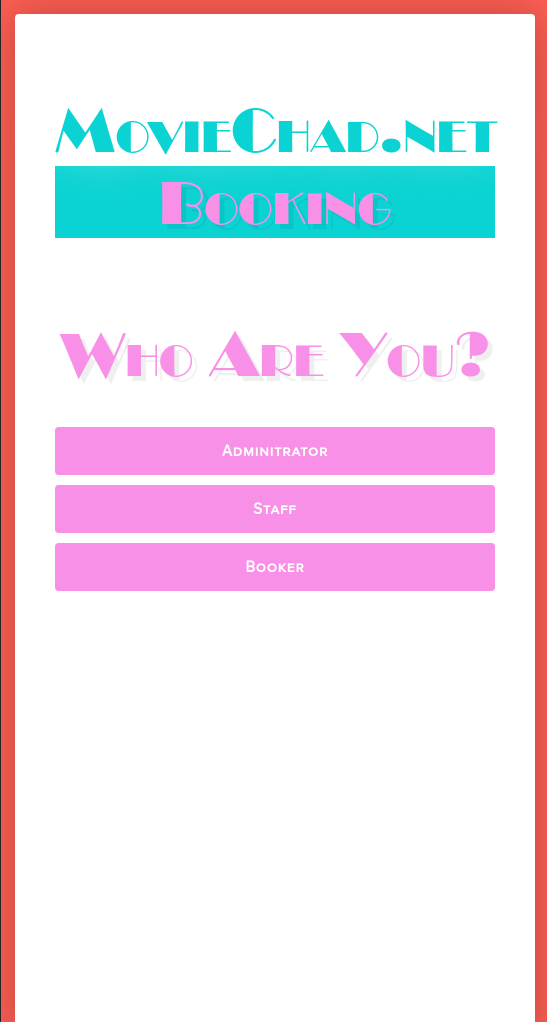
\includegraphics[width=5cm,height=9cm]{CS993_IMG/login1.png} & 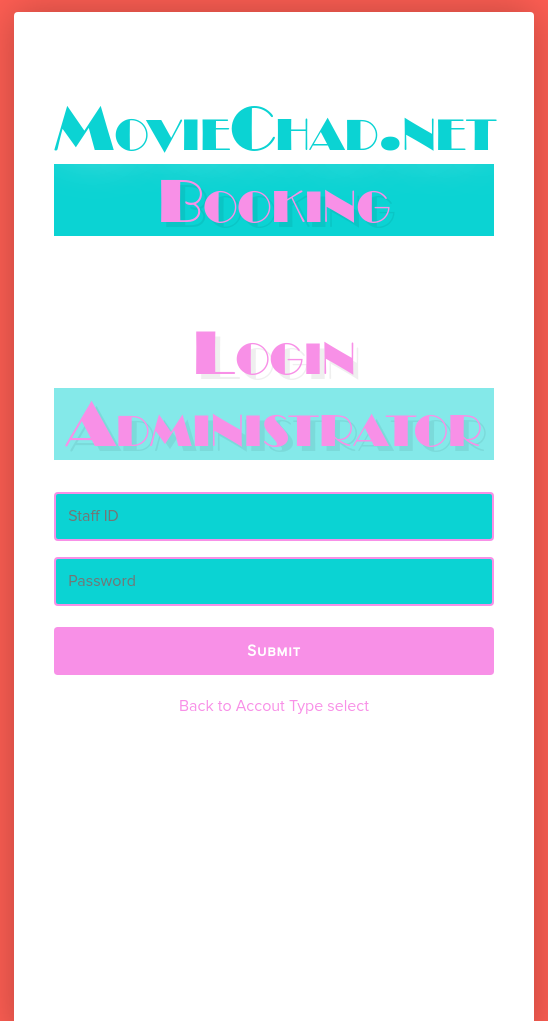
\includegraphics[width=5cm,height=9cm]{CS993_IMG/login2.png} & 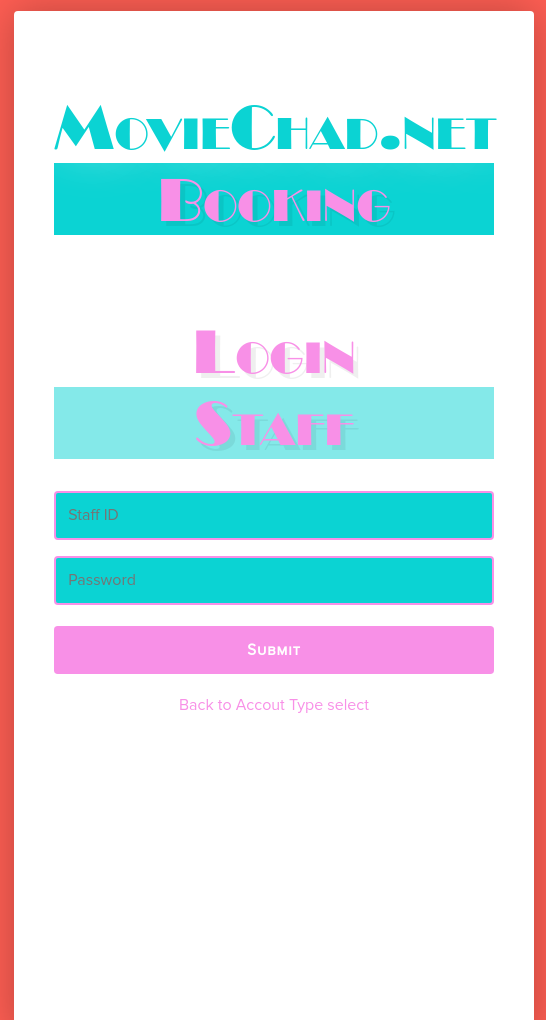
\includegraphics[width=5cm,height=9cm]{CS993_IMG/login7.png}\\
		& \\
		\textbf{Log-In as Booker} & \textbf{Invalid U'name/P'word Demo} & \textbf{Create Account Demo}\\
		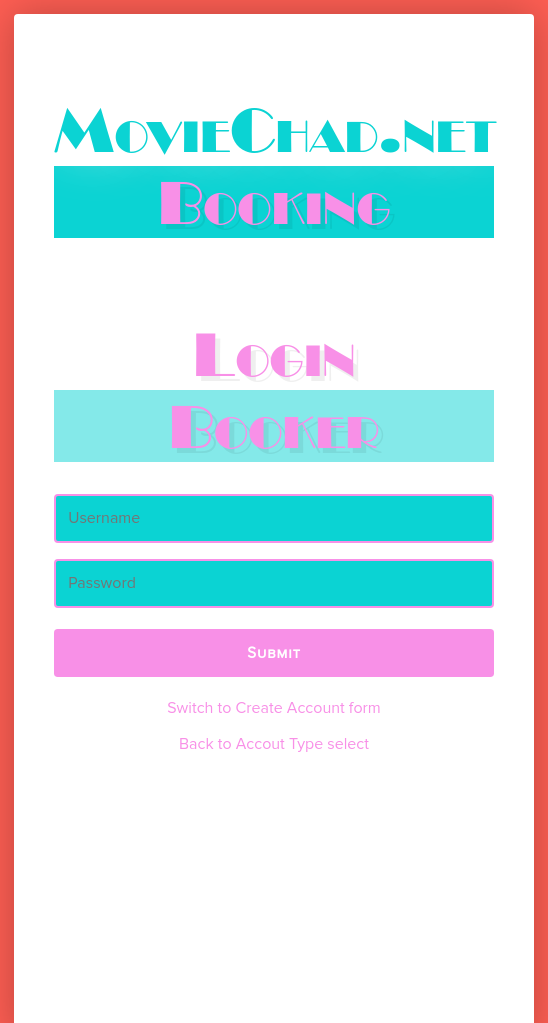
\includegraphics[width=5cm,height=9cm]{CS993_IMG/login3.png} & 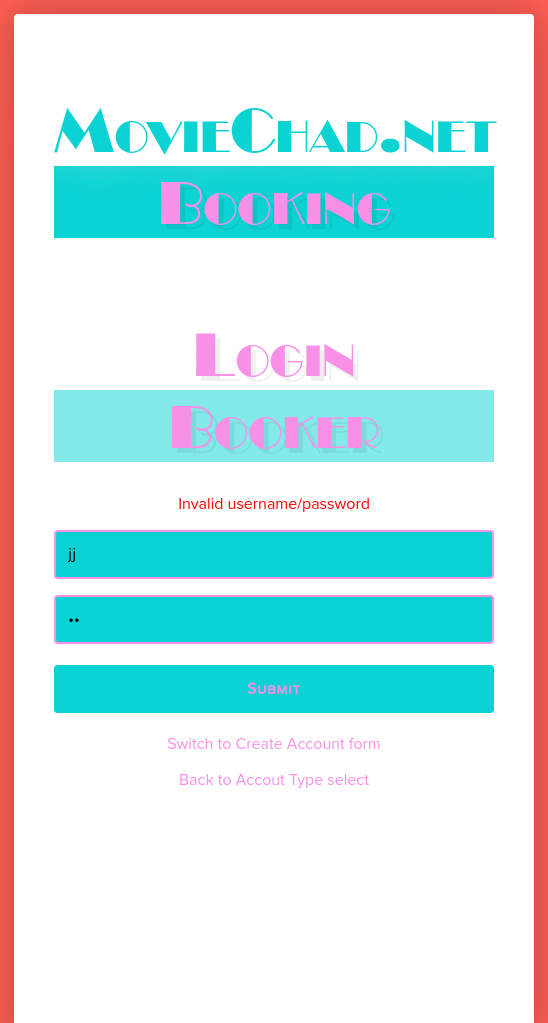
\includegraphics[width=5cm,height=9cm]{CS993_IMG/login4.png} & 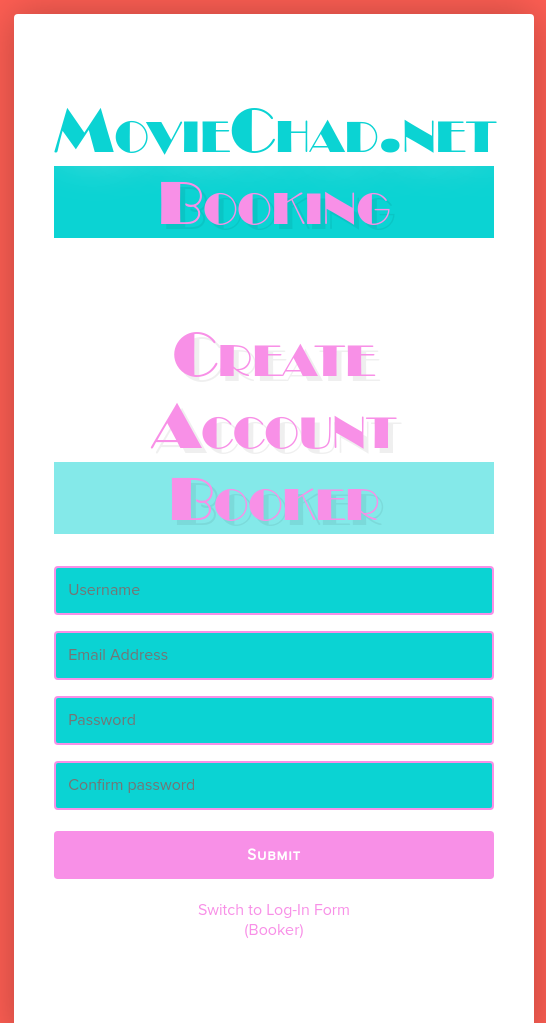
\includegraphics[width=5cm,height=9cm]{CS993_IMG/login5.png}\\
        \end{longtable}
        \end{center}

	\begin{center}
        	\scriptsize
        \begin{longtable}{p{5cm}p{5cm}p{5cm}}
                \textbf{Create Account Errors Demo}\\
		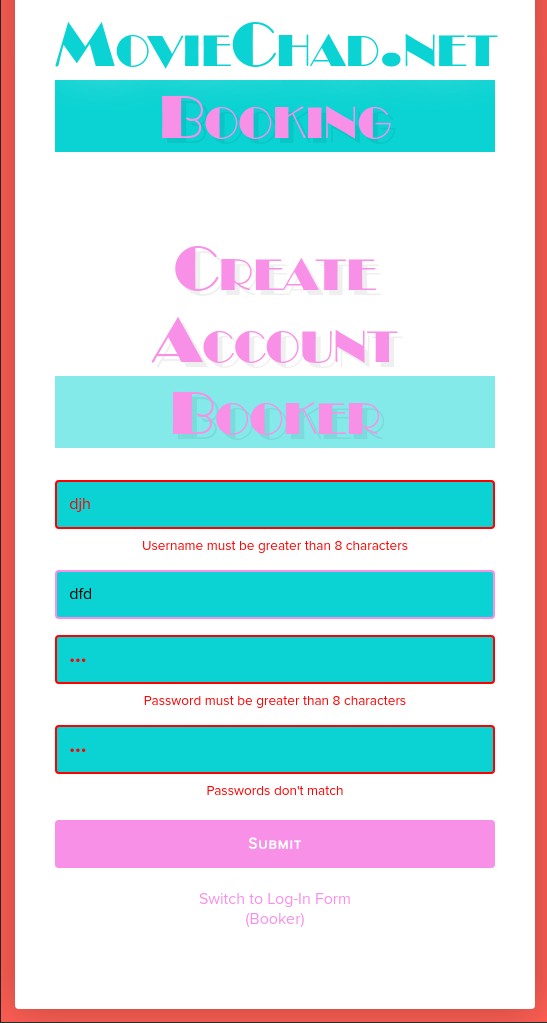
\includegraphics[width=5cm,height=9cm]{CS993_IMG/login6.png}\\
        \end{longtable}
        \end{center}

\newpage

		\subsubsection{Administrator}

	\begin{center}
        	\scriptsize
        \begin{longtable}{p{5cm}p{5cm}p{5cm}}
		\textbf{Add Film Home} & \textbf{Add Film Home (cont.)} & \textbf{Theatre Time Extension}\\
		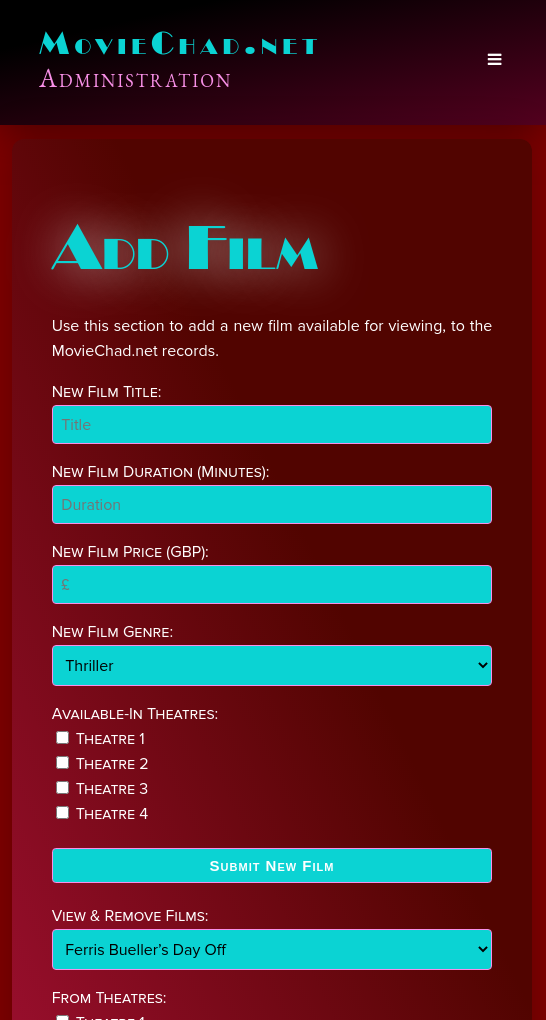
\includegraphics[width=5cm,height=9cm]{CS993_IMG/admin1.png} & 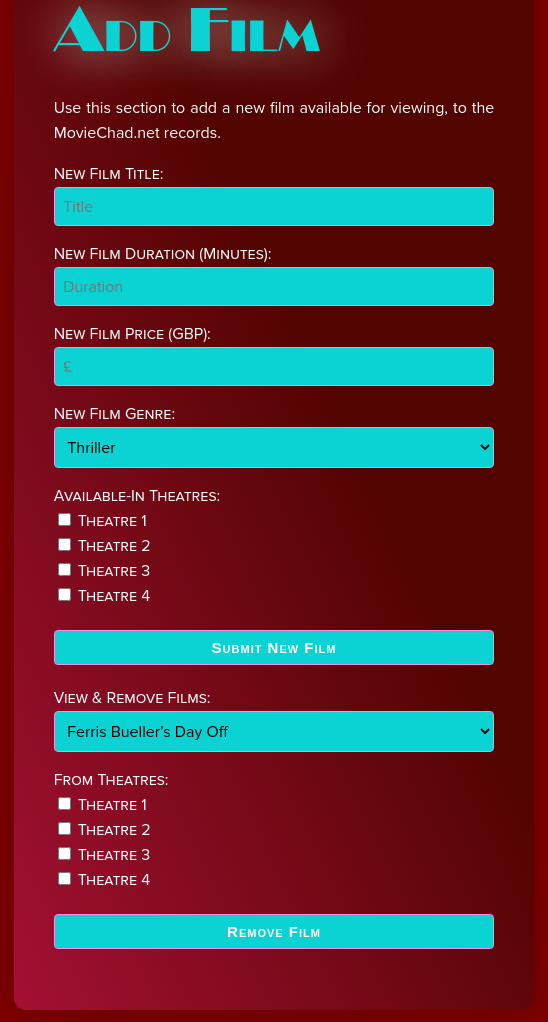
\includegraphics[width=5cm,height=9cm]{CS993_IMG/admin2.png} & 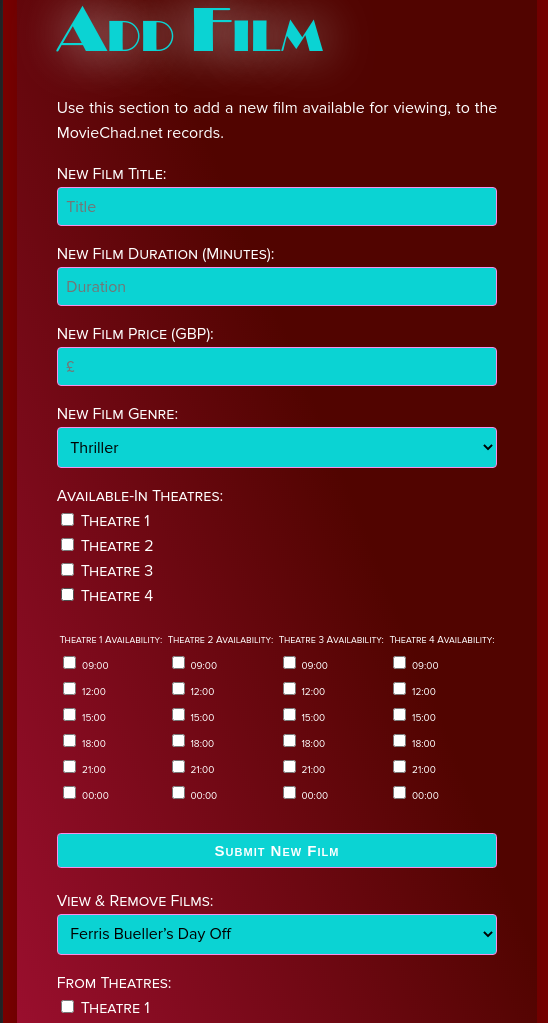
\includegraphics[width=5cm,height=9cm]{CS993_IMG/admin3.png}\\
		& \\
                \textbf{Drop-Down Demo} & \textbf{Check Box Demo} & \textbf{Page Select Drop Demo}\\
		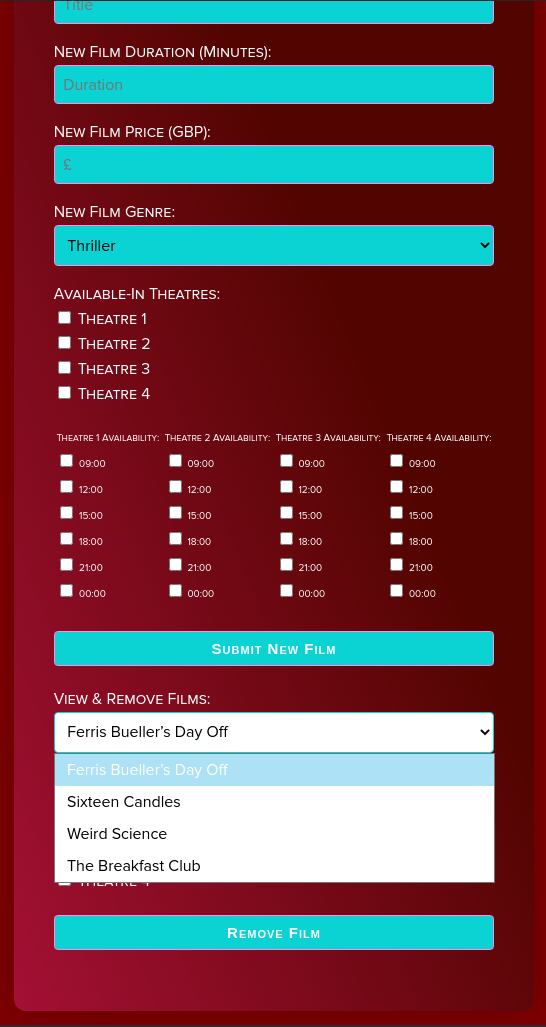
\includegraphics[width=5cm,height=9cm]{CS993_IMG/admin4.png} & 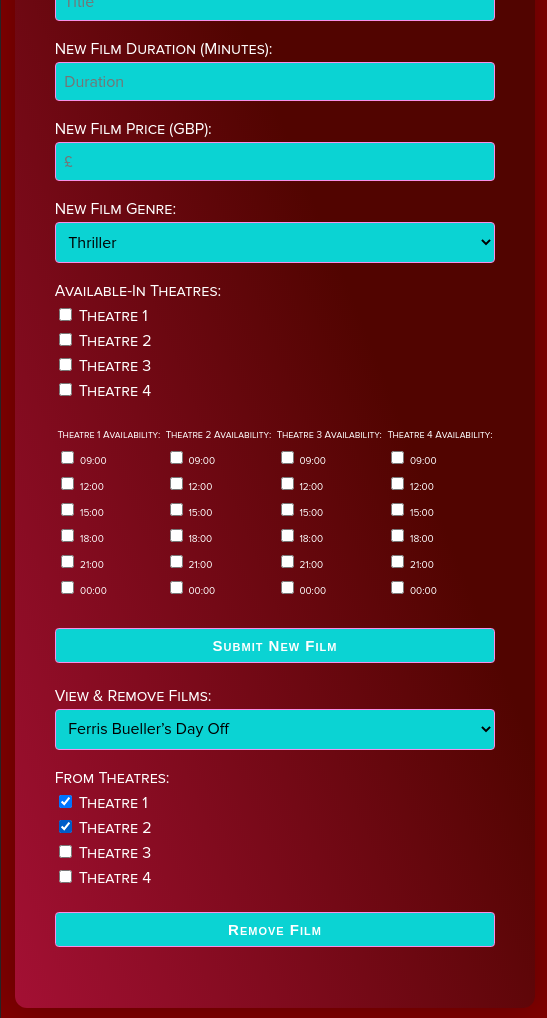
\includegraphics[width=5cm,height=9cm]{CS993_IMG/admin5.png} & 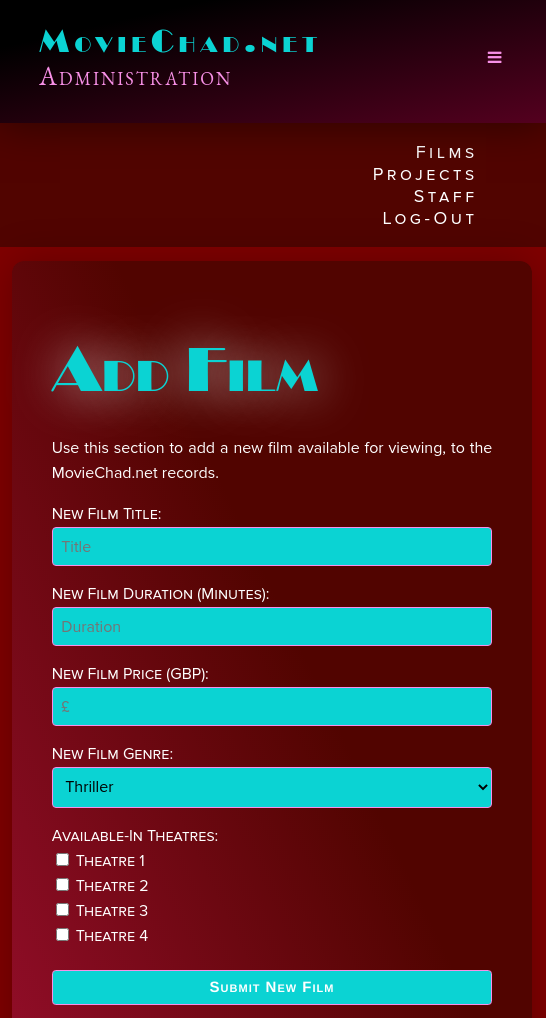
\includegraphics[width=5cm,height=9cm]{CS993_IMG/admin6.png}\\
        \end{longtable}
        \end{center}

\newpage

	\begin{center}
        	\scriptsize
        \begin{longtable}{p{5cm}p{5cm}p{5cm}}
                \textbf{Project Home} & \textbf{Project Expand} & \textbf{Staff Shift Extension}\\
		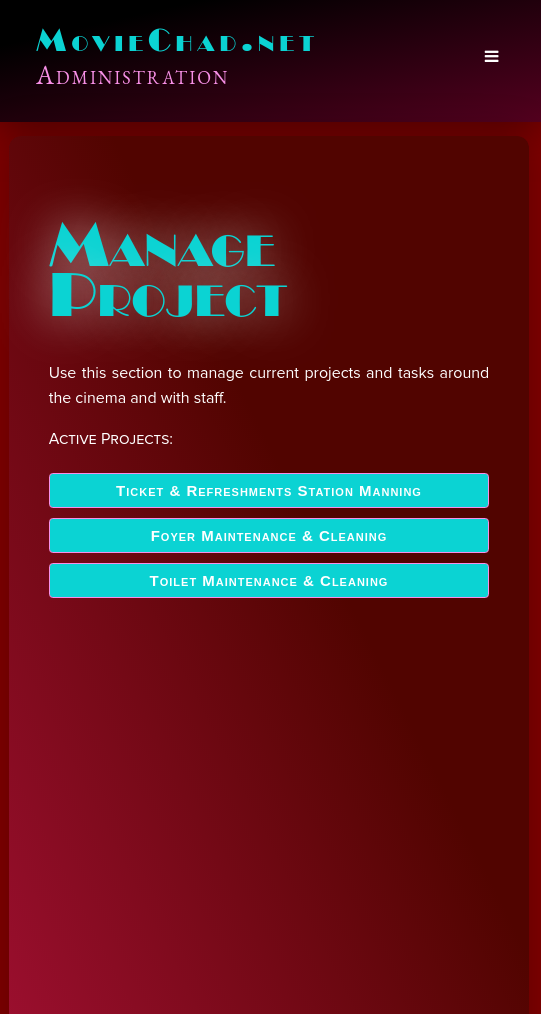
\includegraphics[width=5cm,height=9cm]{CS993_IMG/admin7.png} & 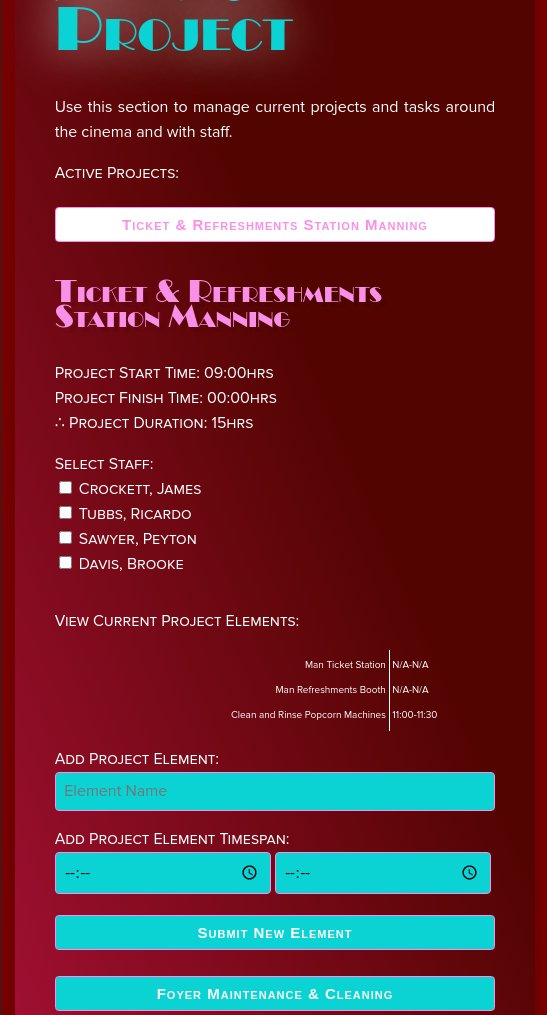
\includegraphics[width=5cm,height=9cm]{CS993_IMG/admin8.png} & 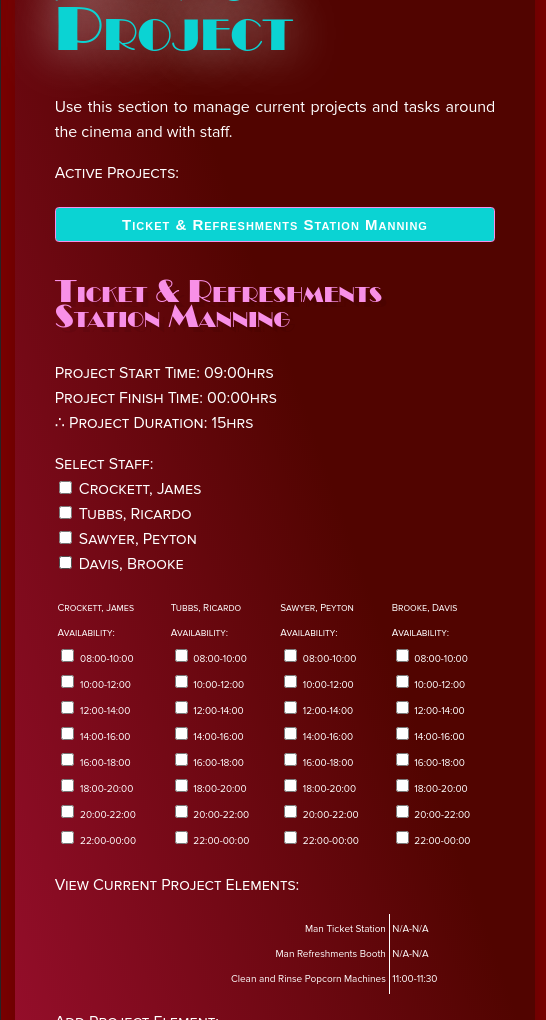
\includegraphics[width=5cm,height=9cm]{CS993_IMG/admin9.png}\\
		& \\
                \textbf{Add Staff Home}\\
		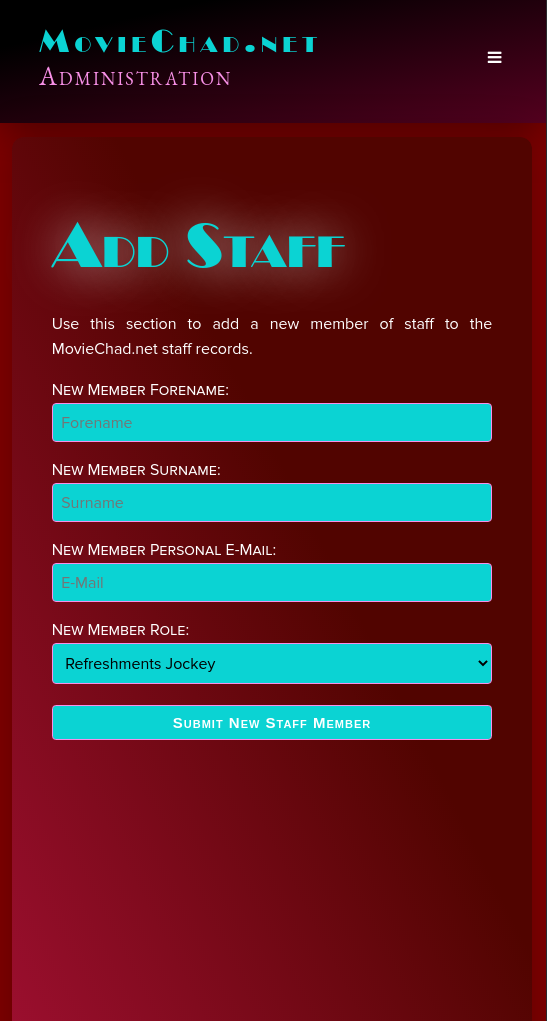
\includegraphics[width=5cm,height=9cm]{CS993_IMG/staff3.png}\\
        \end{longtable}
        \end{center}

\newpage

		\subsubsection{Staff}
		
	\begin{center}
        	\scriptsize
        \begin{longtable}{p{5cm}p{5cm}p{5cm}}
                \textbf{Projects Home} & \textbf{Page Select Drop Demo} & \textbf{Projects Expand}\\
		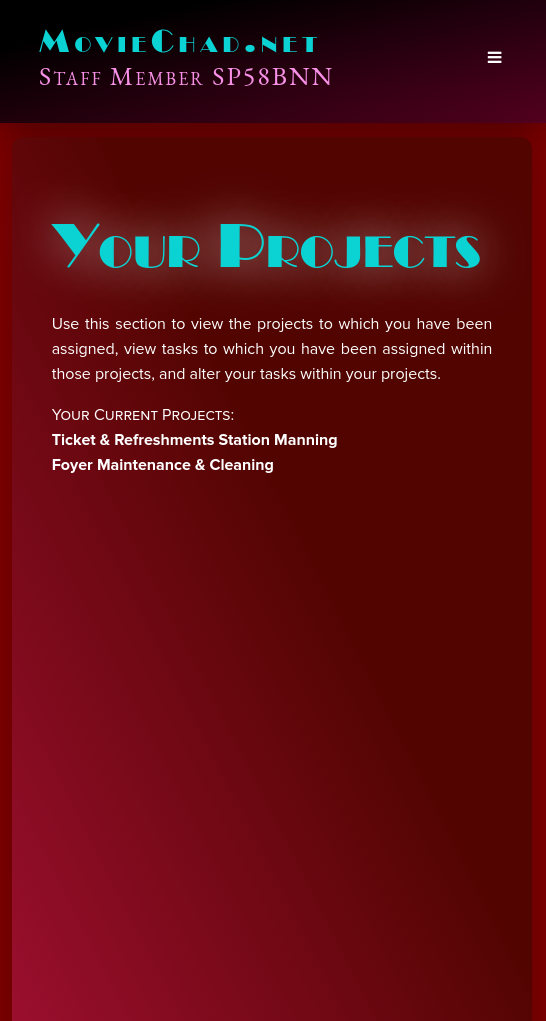
\includegraphics[width=5cm,height=9cm]{CS993_IMG/staff1.png} & 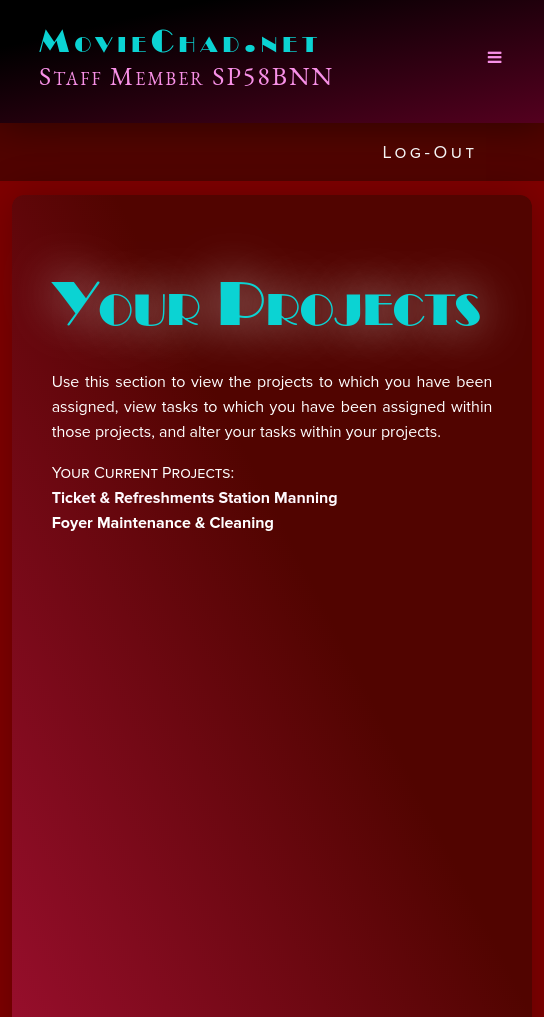
\includegraphics[width=5cm,height=9cm]{CS993_IMG/staff2.png} & 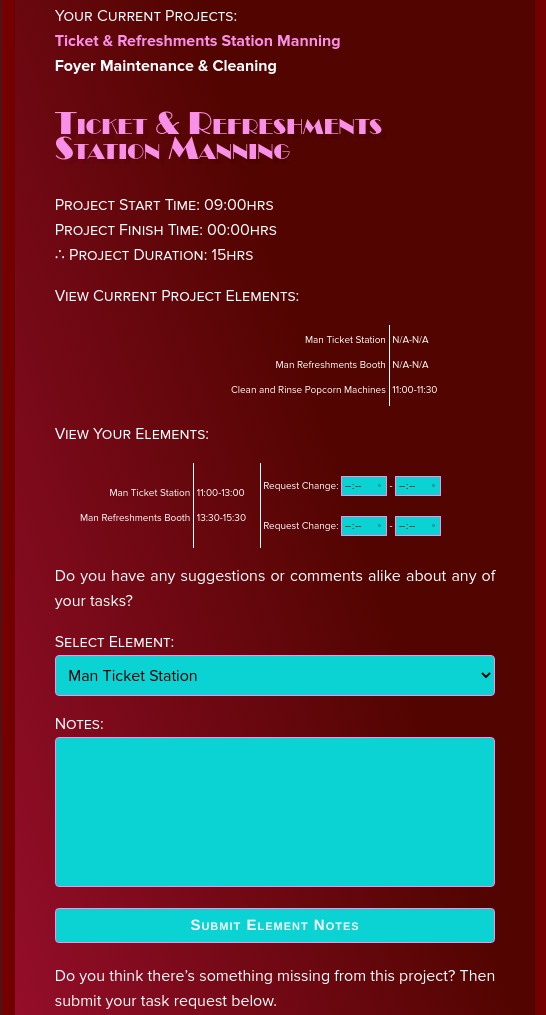
\includegraphics[width=5cm,height=9cm]{CS993_IMG/staff4.png}\\
		& \\
		\textbf{Project Expand (cont.)}\\
		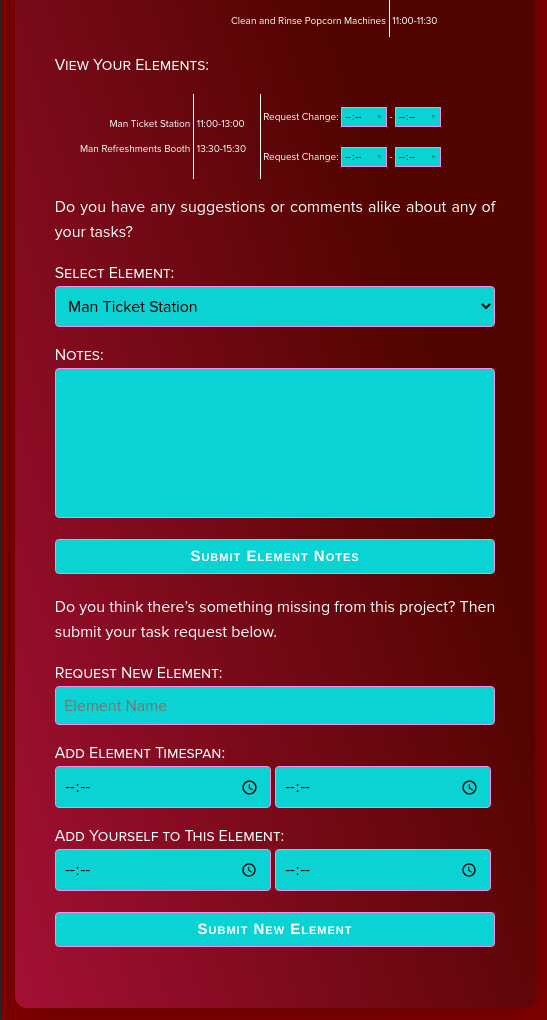
\includegraphics[width=5cm,height=9cm]{CS993_IMG/staff5.png}\\
        \end{longtable}
        \end{center}

\newpage

		\subsubsection{Booker}

	\begin{center}
        	\scriptsize
        \begin{longtable}{p{5cm}p{5cm}p{5cm}}
		\textbf{Theatre 1 Home} & \textbf{Theatre 1 Home (cont.)} & \textbf{Page Select Drop Demo}\\
		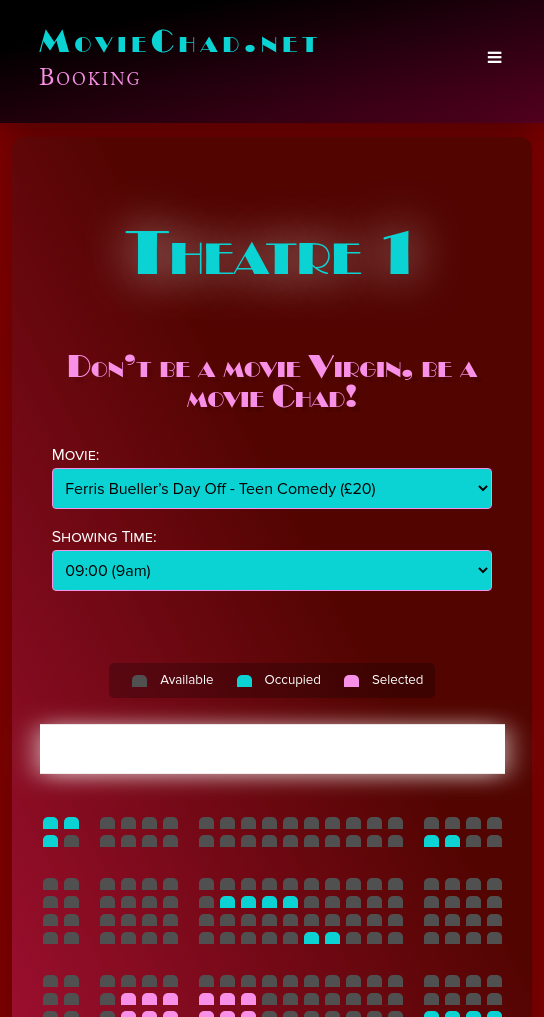
\includegraphics[width=5cm,height=9cm]{CS993_IMG/booker1.png} & 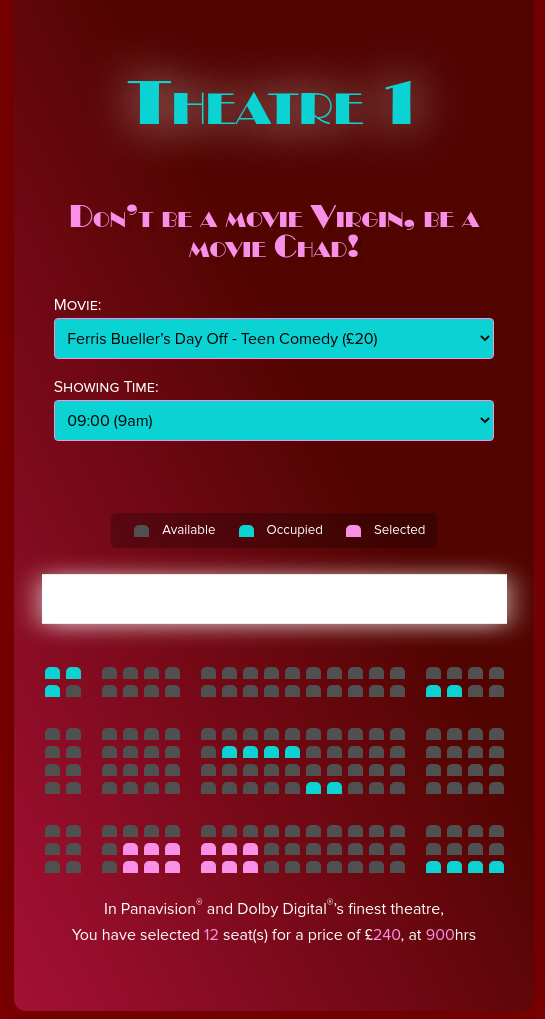
\includegraphics[width=5cm,height=9cm]{CS993_IMG/booker3.png} & 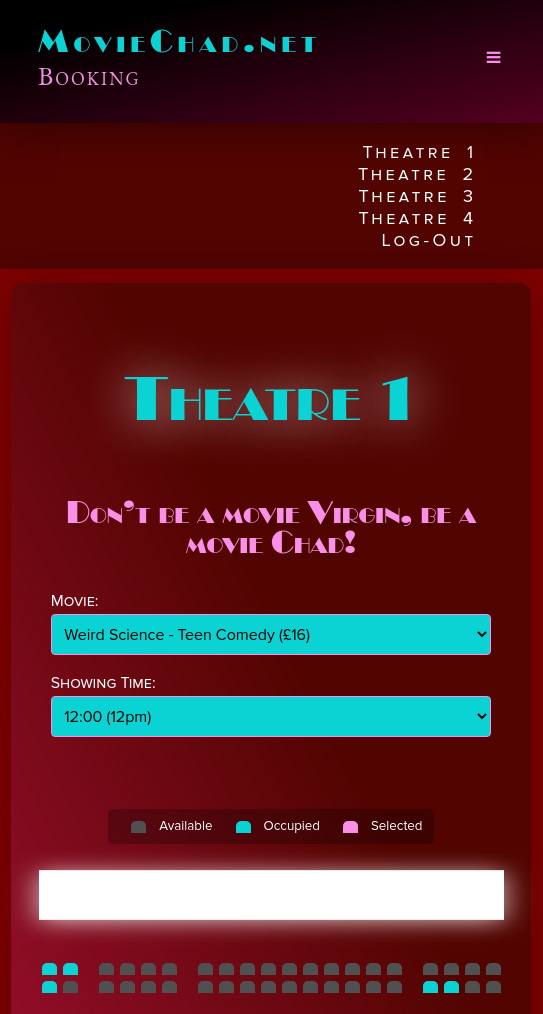
\includegraphics[width=5cm,height=9cm]{CS993_IMG/booker2.png}\\
		& \\
                \textbf{Alter Attributes Demo}\\
		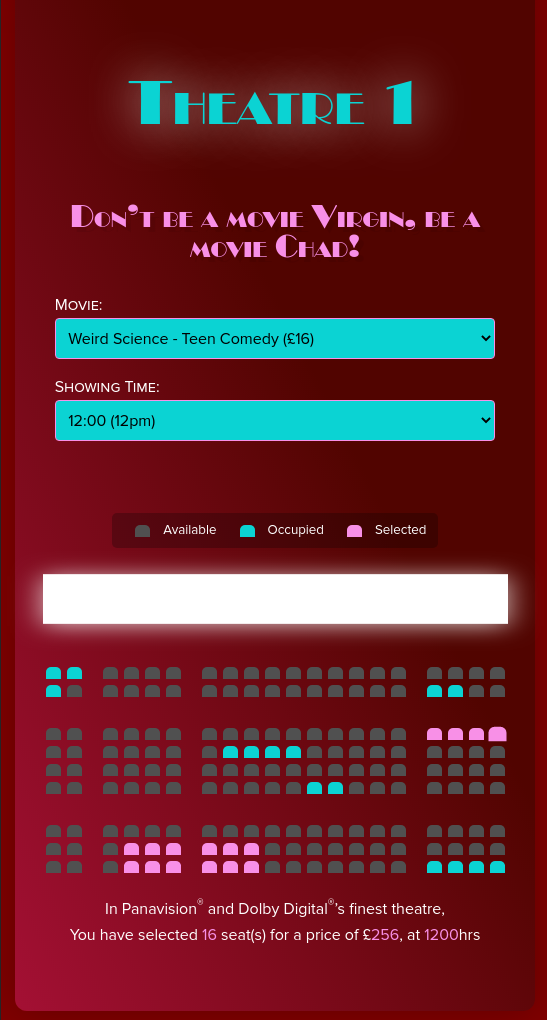
\includegraphics[width=5cm,height=9cm]{CS993_IMG/booker4.png}\\
        \end{longtable}
        \end{center}

	\subsection{Back End}

	The general structure of the rear-end of this system follows the Model View Controller (MVC) pattern, with the caveat that flask uses different naming conventions. The table below outlines this.\\

	\begin{center}
	\begin{tabular}{p{2cm}|p{2cm}p{2.5cm}p{2cm}}
		\textsc{MVC} & MODEL & VIEW & CONTROLLER\\
		\textsc{Flask} & MODEL & TEMPLATES & ROUTER\\
	\end{tabular}
	\end{center}

	The model defines the tables that are stored in the database and the data logic. The templates (views) folder holds the HTML files and is responsible for displaying information to the user. The router file (controller) acts as the bridge between the model and the templates, sending updates from the views the user interacts with to the database as well as updating the views with information received from the models.\\

	Another aspect of the design in structuring the project to make use of Flask's \textit{Application Factories} where an instance of the application is created by a function. While this has its uses for larger applications in terms of running different configurations, in this case the main advantage is the ability to create separate instances of the application when building and running tests. So forth, with regards to the system implementation, the figure below outlines the file structure of the system used in this rear-end. 

	\begin{figure}[H]
        \begin{center}
                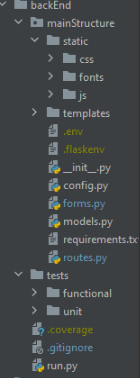
\includegraphics[width=3cm,height=7cm]{CS993_IMG/File_Structure.png}
        \end{center}
        \end{figure}

\newpage

\section{Construction}

	\subsection{Requirements Fulfilment}

	The final construction of this application should see that all of the initially determined requirements and user functionality is implemented correctly and effectively, allowing each user type to take the easiest and most engaging path through their respective portion of the system. With reference to user requirements, recall all which must be implemented:

	\begin{enumerate}
        \setlength\itemsep{0cm}
                \item Account \textit{projects} and \textit{tasks}
                \item Account user roles \textit{administrator} and \textit{`booker'}
                \item Administrators can assign users to projects and tasks
                \item Any user can book time periods against project or task
                \item Any user can add notes (on what \textbf{was} done), and start/finish time
                \item Administrators must log in as administrators
                \item Users must log in as users
                \item Users can only book projects and tasks they're assigned to
                \item Must scale to mobile devices
        \end{enumerate}

	First, the application sees that requirement 1 is met through the inclusion of the administrator and staff roles. Projects, which accounts for primary industrial protocol which takes place in the cinema environment, are created, managed and supervised by administrative users and observed by staff when they're assigned to various aspects. Tasks are also observed within primary protocol as secondary protocol, where each main project is segmented into smaller portions which can be more easily assigned to staff and designated shift patterns, which can also be altered at request by staff.\\

	Further, requirement 2 is met through the inclusion of the discussed user types: admin and staff. In this scenario, the admin takes the administrative role, as implied, and the staff take the booker role, relative to the application brief and specification. Of course, there is a third user in this system, the booker who incidentally does not take the role of a booker as their only role in the system is to fulfil their role in a cinema context. Yes, this could have just been a cinema management system but, the movie booker user allows for the inclusion of further CSS and JavaScript techniques which enhance the comprehensiveness and continuity of the system as a whole.\\

	Requirement 3 is once again fulfilled through the administrator portion of the system, where admins can either select a current, active project to assign staff to specific tasks and time periods (shifts) within. And, they can create new projects, therefore new tasks, through which they can also assign staff to specific tasks and time periods. On the subject, requirement 4 is fulfilled where staff can view their current projects, assigned-to by admins, and the tasks within; and, request shift time changes relative to chosen tasks. Staff also have a section in which they can suggest a new task for the project, meaning all of the element attributes are created by staff and confirmed/denied by admins, in which they can request assignment of themselves to specific shift times. This of course, is also relevant to requirement 4.\\

	Furthermore, staff also have the option and ability to select a task to which they have been assigned upon which they wish to add notes to. This satisfies requirement 5 where staff are prompted to only do this in scenarios where they have relevant feedback regarding their performance, circumstances or suggestions in a particular task after completion. They may also add notes after assignment to highlight any preliminary thoughts etc. This also related to the fulfilment of requirement 8, where members of staff are only permitted to view, suggest shift changes upon, and suggest new tasks for projects to which they have been initially assigned by an administrator in the project creation or maintenance protocol.\\

	Requirements 6 and 7 are both met in the log-in portion of the system, where any user arriving at the site is presented with three options: log-in as an administrator, log-in as a member of staff, or log-in as a movie booker. As previously discussed, it may be considered poor form to include the commercial (movie booker) log-in adjacent to the industrial (administrator and staff) log-in portions however, simplicity and continuity remain the arguments in support of this decision.\\

	Finally, requirement 9 states that the application must scale to mobile devices. As the system's user interface was created using HTML, CSS and JavaScript, clearly it is optimized for web browsers; making it clean, coherent and intuitive to access and navigate for any user type. However in line with requirement 9, various HTML5, CSS and JavaScript elements have been implemented which allow the system to be viewed as a `web application', meaning it cleanly scales to mainstream mobile devices such as mobile telephones and tablets.\\

	The table below sees how the discussed requirements are implemented effectively in the application.

	\begin{center}
		\scriptsize
	\begin{longtable}{p{3cm}p{3cm}p{4cm}p{3cm}}
		\textsc{Element} & \textsc{Function} & \textsc{Functionality} & \textsc{Constraint}\\
		\hline
		\hline
		\multicolumn{4}{c}{\textsc{Log-In Page (index)}}\\
		\hline
		\hline
		\multicolumn{4}{c}{\textsc{Selection Stage 1 (Select Account)}}\\
		\hline
		Link button & Log-in as admin & Hide select account, show admin log-in form & N/A\\
		Link button & Log-in as staff & Hide select account, show staff log-in form & N/A\\
		Link button & Log-in as booker & Hide select account, show booker log-in form & N/A\\
		\hline
		\multicolumn{4}{c}{\textsc{Selection Stage 2.1 (Admin Log-In)}}\\
		\hline
		Text input & Enter admin ID & Relay text & N/A\\
		Text input & Enter admin password & Relay text & N/A\\
		Submit button & Submit login request & Submit inputs, display error upon incorrect text entry & N/A\\
		Link & Back to select account & Hide admin log-in, show select account & N/A\\
		\hline
		\multicolumn{4}{c}{\textsc{Selection Stage 2.2 (Staff Log-In)}}\\
		\hline
		Text input & Enter staff ID & Relay text & N/A\\
		Text input & Enter staff password & Relay text & N/A\\
		Submit button & Submit login request & Submit inputs, display error upon incorrect text entry & N/A\\
		Link & Back to select account & Hide staff log-in, show select account & N/A\\
		\hline
		\multicolumn{4}{c}{\textsc{Selection Stage 2.3 (Booker - Log-In)}}\\
		\hline
		Text input & Enter booker username & Relay text & N/A\\
		Text input & Enter booker password & Relay text & N/A\\
		Submit button & Submit login request & Submit inputs, display error upon incorrect text entry & N/A\\
		Link & Create account & Hide booker log-in, show booker create account & N/A\\
		Link & Back to select account & Hide booker log-in, show select account & N/A\\
		\hline
		\multicolumn{4}{c}{\textsc{Selection Stage 2.3.1 (Booker - Create Account)}}\\
		\hline
		Text input & Enter/choose booker username & Relay text, display error if chosen username string is less than 8 characters & N/A\\
		Text input & Enter/associate booker e-mail & Relay text & N/A\\
		Text input & Enter/choose booker password & Relay text, display error if chosen password string is less than 8 characters & N/A\\
		Text input & Enter/confirm booker password & Relay text, display error if confirm password string is not equal to choose password string & N/A\\
		Submit button & Submit create account request & Submit inputs, do nothing if errors are still displayed & N/A\\
		Link & Back to booker log-in & Hide booker create account, show booker log-in & N/A\\
		\hline
		\hline
		\multicolumn{4}{c}{\textsc{Administration Page (Admin)}}\\
		\hline
		\hline
		Link & Manage films form & Hide manage projects and manage staff, show manage films & N/A\\
		Link & Manage projects form & Hide manage films and manage staff, show manage projects & N/A\\
		Link & Manage staff form & Hide manage films and manage projects, show manage staff & N/A\\
		\hline
		\multicolumn{4}{c}{\textsc{Selection Stage 1.1 (Admin - Films)}}\\
		\hline
		Text input & Add new film title & Relay text & N/A\\
		Number input & Add new film duration (number, `minutes') & Relay number & N/A\\
		Currency input & Add new film price (\pounds\pounds.pp) & Relay number & N/A\\
		Drop-down select & Add new film genre & Relay drop-down selection & N/A\\
		Link checkbox [4] & Choose theatre(s) [1--4] & Show according showings for [1--4] theatres, relay selection(s) & Perhaps not most effective form of link as check boxes lose some CSS functionality when used as links\\
		\hline
		\multicolumn{4}{c}{\textsc{Selection Stage 1.1.1 (Admin - Films - Theatre Time)}}\\
		\hline
		Checkbox [4x6] & Choose showing(s) from [6] times for each [4] theatres & Relay checkbox selection & N/A\\
		\hline
		Submit button & Submit add film request & Submit relevant input to adding a film & N/A\\
		Drop-down select & Choose film title to remove & Relay drop-down selection & N/A\\
		Checkbox [4] & Choose theatre to remove film from & Relay checkbox selection & N/A\\
		Submit button & Submit remove film request & Submit relevant inputs to removing a film & N/A\\
		\\\\\\\\\\\\\\
		\hline
		\multicolumn{4}{c}{\textsc{Selection Stage 2.1 (Admin - Projects)}}\\
		\hline
		Link button [$N$] & Show active project from $N$ available ($\therefore N$ possible buttons) & Show project elements & Keeping the large number of elements involved in a project under one button which can either show or hide them means that if there aren't many projects, a desktop display will not be fully populated when all project elements are contracted\\
		\hline
		\multicolumn{4}{c}{\textsc{Selection Stage 2.1.1 (Admin - Projects - Project)}}\\
		\hline
		Link checkbox [$N$] & Choose staff member(s) [$1-N$] to assign, from $N$ available ($\therefore N$ possible buttons) & Show according shift times for [$1-N$] staff, relay selections & Perhaps not most effective form of link as check boxes lose some CSS functionality when used as links\\
		\hline
		\multicolumn{4}{c}{\textsc{Selection Stage 2.1.1.1 (Admin - Projects - Project - Staff Times)}}\\
		\hline
		Checkbox [$N\times8$] & Choose shift times(s) from [8] times for each [$N$] staff members & Relay checkbox selection & N/A\\
		\hline
		Span [($N,2$)] & Active project elements & Display [$N$] active project element(s) created by admins, by its timescale & N/A\\
		Text input & Add new project element title & Relay text & N/A\\
		Time input & Choose project element start time & Relay time & N/A\\
		Time input & Choose project element end time & Relay time & N/A\\
		Submit button & Submit add element request & Submit relevant inputs to adding a project element & N/A\\
		\hline
		\multicolumn{4}{c}{\textsc{Selection Stage 3.1 (Admin - Staff)}}\\
		\hline
		Text input & Enter new staff member forename & Relay text & N/A\\
		Text input & Enter new staff member surname & Relay text & N/A\\
		Text input & Enter new staff member e-mail address & Relay text & N/A\\
		Drop-down select & Choose new staff member role & Relay drop-down selection & N/A\\
		Submit button & Submit add new staff member request & Relay relevant inputs to adding new staff member & N/A\\
		\hline
		\hline
		\multicolumn{4}{c}{\textsc{Staff Page (Staff)}}\\
		\hline
		\hline
		Span & Staff ID & Display relevant staff ID in header & N/A\\
		\\
		\hline
		\multicolumn{4}{c}{\textsc{Selection Stage 1.1 (Staff - Projects)}}\\
		\hline
		Span [$(N)$] & Assigned projects & List project titles assigned to staff member & N/A\\
		Time input [2] & Request task time change for [2] start and finish & Relay time & N/A\\
		Drop-down select & Choose elements to which notes will be added & Relay drop-down selection & N/A\\
		Text input & Add notes to element once element is completed, the integrity of the `once element is completed' portion is achieved with a written prompt & Relay text & N/A\\
		Submit button & Submit notes on element & Relay text & N/A\\
		Text input & add new project element title & Relay text & N/A\\
		Time input & Choose project element start time & Relay time & N/A\\
		Time input & Choose project element end time & Relay time & N/A\\
		Time input & Choose project element self shift start time & Relay time & N/A\\
		Time input & Choose project element self shift end time & Relay time & N/A\\
		Submit button & Submit add element request & Submit relevant inputs to adding a project element & N/A\\
		\hline
		\hline
		\multicolumn{4}{c}{\textsc{Booker Page (Booker)}}\\
		\hline
		\hline
		\multicolumn{4}{c}{\textsc{Selection Stage 1.1--4.1 - Theatre [1--4]}}\\
		\hline
		\multicolumn{4}{p{13cm}}{\textit{Note that this section of the site contains four identical divisions for theatre bookings therefore, the relevant elements will only be discussed once}}\\
		\hline
		Drop-down select & Choose film title (i.e. film) & Relay drop-down selection & N/A\\
		Drop-down select & Choose film time (i.e. showing time) & Relay drop-down selection & N/A\\
		Div select & Choose seat(s) & Relay class status from division to indicate selection & N/A\\
		Span [3] & Ticket booking element summary & Display total seats selected, total price and showing time selected & N/A\\
		\hline
		\caption{Requirements Functionality}
	\end{longtable}
	\end{center}

	\subsection{Test-Driven Development on Rear-End Functionality}

	Although this stage can only be connected to the interfaceable objects nearer the end of the process, each element must be analysed for practical feasibility as soon as possible. The use of the Agile methodology saw that development of each aspect of the rear-end functionality was actually taking place and being tested according to the evolution and development of new features on the front-end UI. That is, if a new object such as the theatre film showing time selection was being developed on the front-end, a smaller, more manageable and testable version was being developed on the rear-end. This ensures that the concept works and can be adjusted to be fully functional once connected to the front-end object.

	\subsection{Back End Languages \& Technologies}

	For developing the application, consideration of various factors and requirements were taken to ensure that the correct technology stack was selected. The following were included:

	\begin{itemize}
	\setlength\itemsep{0cm}
		\item Initially a small project but could require the ability to scale-up in the future
		\item Ability to quickly develop and deploy the first iteration
		\item As all members of the team had recent experience with SQL and Python, a framework utilizing those technologies would be preferable
		\item Ease of integration with existing prototypes. As they were developed using HTML, CSS and JavaScript, a framework which is able to use these technologies as views would simplify converting the prototypes.
	\end{itemize}

	After consideration of the discussed, the team determined that the web framework Flask was the most suitable option, as:

	\begin{itemize}
	\setlength\itemsep{0cm}
		\item It is lightweight and suitable for small applications, but can be scaled
		\item It is designed to build and deploy web applications quickly
		\item Unlike the most popular Python framework, Django, Flask is considered more `Pythonic', meaning it has a smaller learning curve for those already familiar with Python
		\item Flask uses a templating engine called `Jinja2' which allows the application to dynamically insert data into HTML files
	\end{itemize}

	Due to excellent support for and features provided by Flask projects, the IDE PyCharm was used for rear-end development. For the database, the flask extension Flask-SQLAlchemy was used in tandem with phpMyAdmin.

	\subsection{Version Control}

	Like in any team-based project that involves writing and developing software, version control was used from day one. The team opted for use of GitLab and a remote repository was created which allowed the team to remain up-to-date with all new updates and modifications to the front and back ends made by other members of the team. During development a new feature would be developed in a new branch and once the new functionality was implemented and tested, it would be merged to the main branch.\\

	Using a remote repository gave the team confidence as any local storage issues would not pose threat to the overall project, provided regular commits. And, that it would be easy to trace historic versions when any changes needed to be altered or restored to a previous state.

	\subsection{Application Functionality}

	The state of the application is a working development version of the web application having completed the first sprint. As per the agreed requirements with the client, some of the functionality shown in the prototypes was pushed to later deployments to allow for an earlier release. The application as of this date reflects:

	\begin{itemize}
	\setlength\itemsep{0cm}
		\item A customer (booker) to:
		\begin{itemize}
			\item Sign-up / log-in,
			\item View films currently listed,
			\item Book and receive ticket reservation depending on availability;
		\end{itemize}
		\item and, an administrator to:
		\begin{itemize}
			\item Have the same functionality as the booker,
			\item Create and delete movie listings
		\end{itemize}
	\end{itemize}

		\subsubsection{Sign-Up}

	Users can create an account using the sign-up page by providing an e-mail address, a password, and a confirmation of their password. Various operations such as validation and encryption (bycrypt) are performed to ensure correct and protected data is stored on the database.\\

	As per the figure below of the development database, passwords are shown to be successfully hashed. Note that the \textit{is\_admin} column is used in the router (controller) to determine whether the current user has administrator privileges. The subsequent figure highlights validation at work when attempting a sign-up with an e-mail already stored in the database.

	\begin{figure}[H]
	\begin{center}
		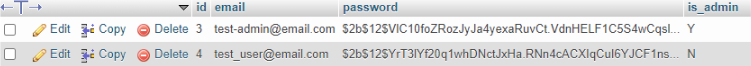
\includegraphics[width=15cm,height=1.5cm]{CS993_IMG/Signup1.png}
		\caption{Sign-Up Structure}
	\end{center}
	\end{figure}

	\begin{figure}[H]
	\begin{center}
		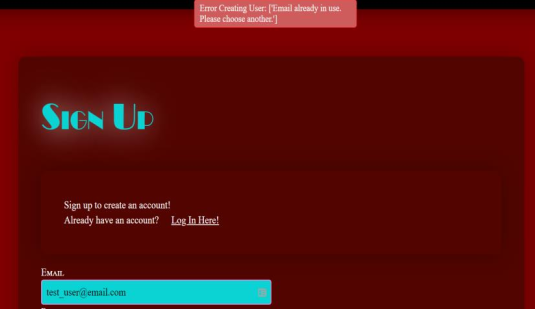
\includegraphics[width=10cm,height=6cm]{CS993_IMG/Signup2.png}
		\caption{Account Exists Example}
	\end{center}
	\end{figure}

		\subsubsection{Log-In}

	Once registered, users (or the existing administrator) can log-in through the log-in page using their e-mail address and password. Validation is active on the forms to inform the user of any errors in their log-in attempt.

		\subsubsection{Reserve Tickets}

	Once logged in, all users are redirected to the home page where they can select a single film and the number of tickets they would like to reserve (maximum of 5). If successful, they are redirected to a page confirming their reservation with details of the number of tickets, total price, and instructions to present the ticket once arriving at the cinema to complete their purchase. The number of tickets reserved is noted and the movie table in the database is updated to decrease the number of available tickets, if users attempt to reserve more tickets than are available, they are redirected to the homepage with an error stating the fact. The below figure shows a snapshot of the movies table in the database.

	\begin{figure}[H]
	\begin{center}
		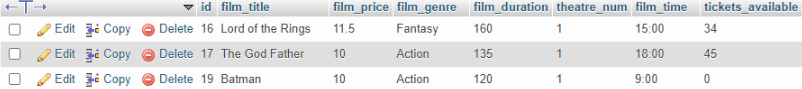
\includegraphics[width=14cm,height=1.5cm]{CS993_IMG/Reserve.png}
		\caption{Reserve Tickets Structure}
	\end{center}
	\end{figure}

		\subsubsection{Creating \& Deleting Movies}

	Once the administrator logs in, they will have all the functionality of the customer as well as having the ability to create and delete movies through the add movie page.

		\subsubsection{Route Protection \& Admin Privileges}

	The flask module, `flask-login' includes functionality (using CSRF tokens) to ensure that certain routes within the application can only be accessed by authenticated users. The authentication and administrator status of the user is passed on to the views, and a conditional in the navigation (HTML/Jinja2) determines which navigation links are visible to the current user. This is outlined in the demonstrations within the following two figures.

	\begin{figure}[H]
	\begin{center}
		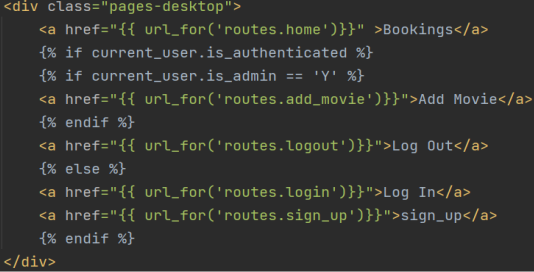
\includegraphics[width=8cm,height=3.5cm]{CS993_IMG/Route1.png}
		\caption{Route Protection \& Admin Privileges 1}
	\end{center}
	\end{figure}

	\begin{figure}[H]
	\begin{center}
		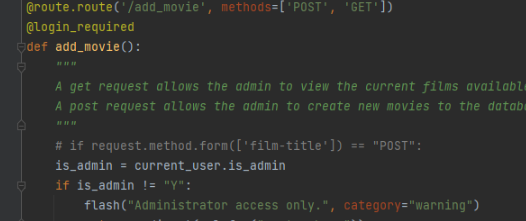
\includegraphics[width=8cm,height=3cm]{CS993_IMG/Route2.png}
		\caption{Route Protection \& Admin Privileges 2}
	\end{center}
	\end{figure}

\newpage

\section{Testing}

	It was important that from the first day of the project that a well thought out approach and implementation of testing would be a priority. Accomplishing this prevents an accumulation of `technical debt' where issues are delayed and/or not identified and attempting to solve these issues later could bottleneck the development process. Unit testing and systems testing were performed throughout development, and user acceptance testing was the final hurdle to accomplish before passing the application over to the client.

	\subsection{Unit Testing}

The first step of testing involved using unit tests to test the each of the small parts of the code base (units) independently of each other.\\

Flask is compatible with the Python testing module `Pytest' which allowed us to easily write unit tests. The following is a unit test that was written to test the logic when creating a user. The test follows the `GIVEN-WHEN-THEN' approach to describe a test which helps to ensure tests are written in well structured, well purposed manner:
		
	\begin{itemize}
	\setlength\itemsep{0cm}
		\item Given - What are the conditions?
		\item When - What is being tested?
		\item Then - What is the expected outcome?
	\end{itemize}

	Unit tests were easily run in the terminal, as shown in the following two figures.

	\begin{figure}[H]
	\begin{center}
		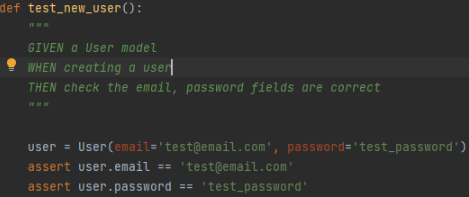
\includegraphics[width=8cm,height=3cm]{CS993_IMG/Testing1.png}
		\caption{Unit Testing Example 1}
	\end{center}
	\end{figure}

	\begin{figure}[H]
	\begin{center}
		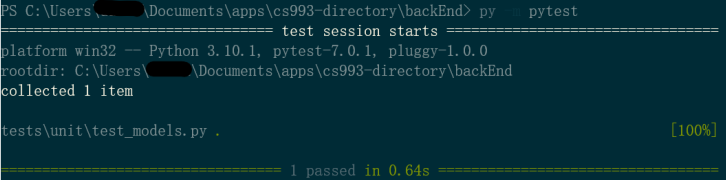
\includegraphics[width=12cm,height=3cm]{CS993_IMG/Testing2.png}
		\caption{Unit Testing Example 2}
	\end{center}
	\end{figure}

	An additional testing package `pytest-cov' was used to determine how much of the codebase was covered by tests which informed the team where levels of testing were adequate and where more testing was required.

	\begin{figure}[H]
	\begin{center}
		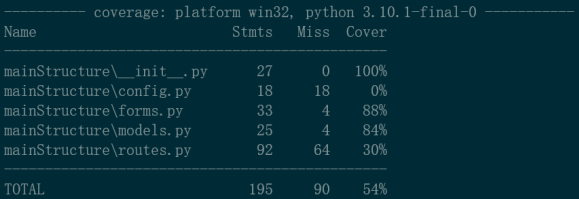
\includegraphics[width=10cm,height=3cm]{CS993_IMG/Testing3.png}
		\caption{Unit Testing Example 3}
	\end{center}
	\end{figure}

	\subsection{Systems Testing}

	Systems testing was undertaken to confirm that the application's functionality was still in line with the functional and non-functional requirements, this was achieved by undertaking functional testing and usability testing.\\

	As discussed earlier in the design section, the approach to developing the application using an `application factory' would allow us to create an instance of the application for testing purposes. This allowed us to test user requirements, an example being to ensure unauthorized users cannot access protected routes.

	\begin{figure}[H]
	\begin{center}
		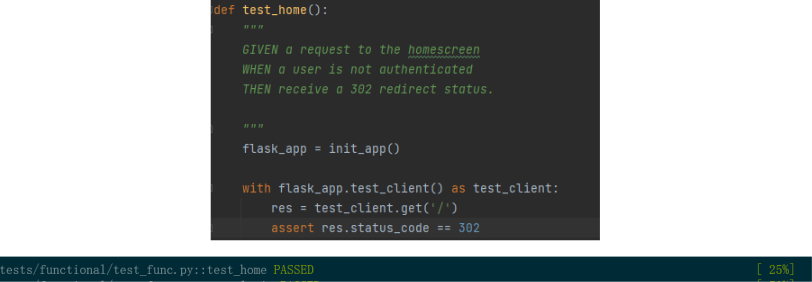
\includegraphics[width=14cm,height=5cm]{CS993_IMG/Testing4.png}
		\caption{Systems Testing Example}
	\end{center}
	\end{figure}

	\subsection{Usability Testing}

	After each iteration we took seven users and presented them with our system on either a mobile or desktop device. We observed these users as they interacted with the system and then interviewed them afterwards on their experience. In the interviews we asked the users a mix of open and closed questions to gather a good mix of qualitative and quantitative data on their experiences.We used new users for each round of testing to ensure there was no familiarity bias arising from certain people already having used an earlier iteration of the system.\\

	Both the observations and interviews provided vital feedback on our implementation of the system, particularly around the UI. In tandem with our other testing methods, the information gathered from these test users was extremely helpful in steering our revised requirements for each proceeding sprint.\\

	Some quantitative results from the user interviews included:

	\begin{figure}[H]
        \begin{center}
                \begin{subfigure}[t]{6cm}
                \begin{center}
                        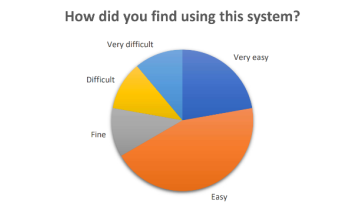
\includegraphics[width=6cm,height=3.5cm]{CS993_IMG/Testing5.png}
                \end{center}
                        \caption{Usability}
                \end{subfigure}
                \begin{subfigure}[t]{6cm}
                \begin{center}
                        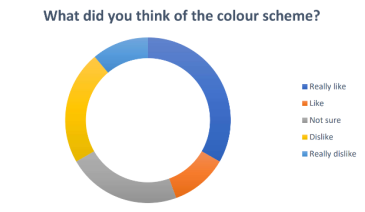
\includegraphics[width=6cm,height=3.5cm]{CS993_IMG/Testing6.png}
                \end{center}
                        \caption{Colour Scheme}
                \end{subfigure}
        \end{center}
		\caption{Quantitative Response}
        \end{figure}

	Some qualitative results, in response to the question: ``what do you think of this system?'', from the user interviews included:

	\begin{itemize}
        \setlength\itemsep{0cm}
		\item I like the look of it, the retro feel is very cool
		\item It's quite easy to use
		\item It's clear how to work it, but I would like some more pictures
		\item The colours are nice and bold
		\item I'd like more information on the movies before booking
	\end{itemize}

	\subsection{User Acceptance Testing}

	Finally, before deploying the first iteration of the application user acceptance testing (UAT) was undertaken. This was the final stage of testing as UAT testing can only take place once all other forms of testing have been completed. The client was involved in each step of the process as the aim of UAT is to ensure the system meets their requirements.\\

	Firstly, a plan was drawn up to outline the process and expectations. The team then designed the UAT test cases, these were mainly determined by the user stories defined in the requirements specification. The tests were then run in a production-like environment by a pre-selected team comprised of some members of development team and the client and any issues/defects were documented. The team then went through the documented issues resolving each one and finally once the client was satisfied, the project was signed off.

\end{document}
